%==================================================================================================
\chapter{Robot localization}

%==================================================================================================
\section{Baisc concepts in robot localisation}

%--------------------------------------------------------------------------------------------------
\subsection{Sensors}
There are a wide variety of sensors used in mobile robots (figure 4.1). Some sensors are
used to measure simple values like the internal temperature of a robot’s electronics or the
rotational speed of the motors. Other, more sophisticated sensors can be used to acquire
information about the robot’s environment or even to directly measure a robot’s global
position. In this chapter we focus primarily on sensors used to extract information about the
robot’s environment. Because a mobile robot moves around, it will frequently encounter
unforeseen environmental characteristics, and therefore such sensing is particularly critical.
We begin with a functional classification of sensors. Then, after presenting basic tools for
describing a sensor’s performance, we proceed to describe selected sensors in detail.
We classify sensors using two important functional axes: proprioceptive/exteroceptive and
passive/active.
\begin{itemize}
	\item Proprioceptive sensors measure values internal to the system like a motor speed or
		battery voltage,
	\item Exteroceptive sensors acquire information from the robot environment like a distance
		to obstacle, 
	\item Passive sensors measure external signals interacting with them, for example cameras
		that detect light reflected from objects,
	\item Active sensors emit signals into the environment, then measure it reaction, for example
		a sonar will emit ultrasound wave and measure time after which it will return to source. 
\end{itemize}
As active sensors provide a  more controlled interactions with the environment, they  will be
preffered in most cases. However, this approach is not without a downsides:
\begin{itemize}
	\item the outbound energy may affect the very characteristics that the sensor is attempting
		to measure, 
	\item interference between emitted signal and other signal of similar nature, for 
		example generated by other robot, may cause errors.
\end{itemize}
Mobile robots depend heavily on exteroceptive sensors. Many of these sensors concentrate
on a central task for the robot: acquiring information on objects in the robot’s immediate
vicinity so that it may interpret the state of its surroundings. Of course, these ``objects'' 
surrounding the robot are all detected from the viewpoint of its local reference frame. Since
the analyzed systems are mobile, their ever-changing position and their motion have a 
significant impact on overall sensor behavior.
Blurring of systematic and random errors. Active ranging sensors tend to have failure
modes that are triggered largely by specific relative positions of the sensor and environment
targets. For example, a sonar sensor will produce specular reflections, producing grossly
inaccurate measurements of range, at specific angles to a smooth sheetrock wall. During
motion of the robot, such relative angles occur at stochastic intervals. This is especially true
in a mobile robot outfitted with a ring of multiple sonars. The chances of one sonar entering
this error mode during robot motion is high. From the perspective of the moving robot, the
sonar measurement error is a random error in this case. Yet, if the robot were to stop,
becoming motionless, then a very different error modality is possible. If the robot’s static
position causes a particular sonar to fail in this manner, the sonar will fail consistently and
will tend to return precisely the same (and incorrect!) reading time after time. Once the
robot is motionless, the error appears to be systematic and of high precision.
The fundamental mechanism at work here is the cross-sensitivity of mobile robot sensors to robot
pose and robot-environment dynamics. The models for such cross-sensitivity
are not, in an underlying sense, truly random. However, these physical interrelationships
are rarely modeled and therefore, from the point of view of an incomplete model, the errors
appear random during motion and systematic when the robot is at rest.
Sonar is not the only sensor subject to this blurring of systematic and random error
modality. Visual interpretation through the use of a CCD camera is also highly susceptible
to robot motion and position because of camera dependence on lighting changes, lighting
specularity (e.g., glare), and reflections. The important point is to realize that, while 
systematic error and random error are well-defined in a controlled setting, the mobile robot can
exhibit error characteristics that bridge the gap between deterministic and stochastic error
mechanisms.

%--------------------------------------------------------------------------------------------------
\subsection{Error modeling}
Multimodal error distributions. It is common to characterize the behavior of a sensor’s
random error in terms of a probability distribution over various output values. In general,
one knows very little about the causes of random error and therefore several simplifying
assumptions are commonly used. For example, we can assume that the error is zero-mean,
in that it symmetrically generates both positive and negative measurement error. We can
go even further and assume that the probability density curve is Gaussian. Although we discuss 
the mathematics of this in detail in section 4.2, it is important for now to recognize the
fact that one frequently assumes symmetry as well as unimodal distribution. This means
that measuring the correct value is most probable, and any measurement that is further
away from the correct value is less likely than any measurement that is closer to the correct
value. These are strong assumptions that enable powerful mathematical principles to be
applied to mobile robot problems, but it is important to realize how wrong these assumptions 
usually are.
Consider, for example, the sonar sensor once again. When ranging an object that reflects
the sound signal well, the sonar will exhibit high accuracy, and will induce random error
based on noise, for example, in the timing circuitry. This portion of its sensor behavior will
exhibit error characteristics that are fairly symmetric and unimodal. However, when the
sonar sensor is moving through an environment and is sometimes faced with materials that
cause coherent reflection rather than returning the sound signal to the sonar sensor, then the
sonar will grossly overestimate the distance to the object. In such cases, the error will be
biased toward positive measurement error and will be far from the correct value. The error
is not strictly systematic, and so we are left modeling it as a probability distribution of
random error. So the sonar sensor has two separate types of operational modes, one in
which the signal does return and some random error is possible, and the second in which
the signal returns after a multipath reflection, and gross overestimation error occurs. The
probability distribution could easily be at least bimodal in this case, and since overestimation 
is more common than underestimation it will also be asymmetric.
As a second example, consider ranging via stereo vision. Once again, we can identify
two modes of operation. If the stereo vision system correctly correlates two images, then
the resulting random error will be caused by camera noise and will limit the measurement
accuracy. But the stereo vision system can also correlate two images incorrectly, matching
two fence posts, for example, that are not the same post in the real world. In such a case
stereo vision will exhibit gross measurement error, and one can easily imagine such behavior 
violating both the unimodal and the symmetric assumptions.
The thesis of this section is that sensors in a mobile robot may be subject to multiple
modes of operation and, when the sensor error is characterized, unimodality and symmetry
may be grossly violated. Nonetheless, as we shall see, many successful mobile robot systems 
make use of these simplifying assumptions and the resulting mathematical techniques
with great empirical success.
The above sections have presented a terminology with which we can characterize the
advantages and disadvantages of various mobile robot sensors. In the following sections,
we do the same for a sampling of the most commonly used mobile robot sensors today.

%--------------------------------------------------------------------------------------------------
\subsection{Relative localisation versus dead reckoning}

%--------------------------------------------------------------------------------------------------
\section{Radio beacon localisation}

%--------------------------------------------------------------------------------------------------
\subsection{Beacon as a reference point}
All Global Satellite Navigation systems (GNSS) are variant of beacon-based localization
systems\cite{Blewitt1997}. Such systems require information about the beacon position
and distance between the localized object and beacons.
With that information, it is possible to calculate the position of an object in the same reference
frame as that of beacons.
Both of those tasks are much more difficult in GNSS due to the nature of the beacons.
Unlike in the case of stationary beacons, GNSS satellites move at high speed so
their position must be calculated based on satellite ephemerides.
Another problem is how to measure distance with use of reasonably priced reciever while 
maintaining high level of precision.
There are three possible approaches to a beacon based localisation:
\begin{itemize}
	\item Time of Arrival (ToA),
	\item Angle of Arrival (AoA),
	\item Received Signal Strength (RSS).
\end{itemize}
AoA detects at which angle a beacon signal arrives and reqires a specialised receiver capable 
of such measurements. This type of localization requires a complex reciever and do not provide 
a satisfactionary precision when dealing with such remote objects as a satellites.
While RSS can work with a very simple reciever its precision is low for signals that, like
the GPS signal, are designed with low power loss over large distances.
This leaves ToA as only valid solution, when measuring distance by ToA 
three properties of a signal should be known:
\begin{itemize}
	\item $t_o$ - time of origination,
	\item $t_a$ - time of arrival,
	\item $v$ - velocity.
\end{itemize}
In case of GNSS signal is an electromagnetic wave therefore its speed is equal
to a speed of light $c$. Time of arrival is recorded when
data frame wavefront reaches the receiver, this means that receiver time is used.
Signal generation time is recorded on satellite according to its local clock and
included in the data frame. Thanks to that distance can be calculated by simple
equation:
\begin{equation}
	d=c(t_a-t_o).
\end{equation}
However $t_a$ and $t_o$ are using different reference frame so for comparison
to be possible they must be transformed into a common reference frame.
This is referred to as a synchronization of the clocks and is very important as
a desynchronization on the level of a single nanosecond results in about 30 cm of
positioning error\cite{Enge2011}.
With distance to beacons measured a trilateration can be used to determine position.


%--------------------------------------------------------------------------------------------------
\subsection{Two point trilateration}
True-range multilateration is a method to determine the location of a movable vehicle or
stationary point in space using multiple ranges (distances) between the vehicle/point and 
multiple spatially-separated known locations (often termed 'stations'). 
The name is derived from trilateration, the geometrical problem of determining an unknown 
position on a plane based on the distance to other two known vertices of a triangle 
(the length of two sides). 
True range multilateration is both a mathematical topic and an applied technique used in several
fields. 
A practical application involving a fixed location is the trilateration method of surveying.
Applications involving vehicle location are termed navigation when on-board persons/equipment are 
informed of its location, and are termed surveillance when off-vehicle entities are informed of 
the vehicle's location.
Two slant ranges from two known locations can be used to locate a third point in a two-dimensional 
Cartesian space (plane), which is a frequently applied technique (e.g., in surveying). 
Similarly, two spherical ranges can be used to locate a point on a sphere, which is a fundamental 
concept of the ancient discipline of celestial navigation — termed the altitude intercept problem.
Moreover, if more than the minimum number of ranges are available, it is good practice to utilize 
those as well. This article addresses the general issue of position determination using multiple 
ranges.
In two-dimensional geometry, it is known that if a point lies on two circles, then the circle 
centers and the two radii provide sufficient information to narrow the possible locations down to 
two – one of which is the desired solution and the other is an ambiguous solution.
Additional information often narrow the possibilities down to a unique location. 
In three-dimensional geometry, when it is known that a point lies on the surfaces of three 
spheres, then the centers of the three spheres along with their radii also provide sufficient 
information to narrow the possible locations down to no more than two (unless the centers lie on 
a straight line).
True range multilateration can be contrasted to the more frequently encountered (pseudorange) 
multilateration, which employs range differences to locate a (typically, movable) point. 
Pseudo range multilateration is almost always implemented by measuring times-of-arrival (TOAs) 
of energy waves. True range multilateration can also be contrasted to triangulation, 
which involves the measurement of angles.
Multiple, sometimes overlapping and conflicting terms are employed for similar concepts – e.g., 
multilateration without modification has been used for aviation systems employing both true ranges
and pseudo ranges. Moreover, different fields of endeavor may employ different terms. 
In geometry, trilateration is defined as the process of determining absolute or relative locations 
of points by measurement of distances, using the geometry of circles, spheres or triangles.
In surveying, trilateration is a specific technique. The term true range multilateration is 
accurate, general and unambiguous. Authors have also used the terms range-range and rho-rho 
multilateration for this concept.
Two Cartesian dimensions, two measured slant ranges (Trilateration). 
An analytic solution has likely been known for over 1,000 years, and is given in several texts.
Moreover, one can easily adapt algorithms for a three dimensional Cartesian space.
The simplest algorithm employs analytic geometry and a station-based coordinate frame.
\begin{figure}[htb] 
	\label{fig:two_beacon_local}
	\centering
	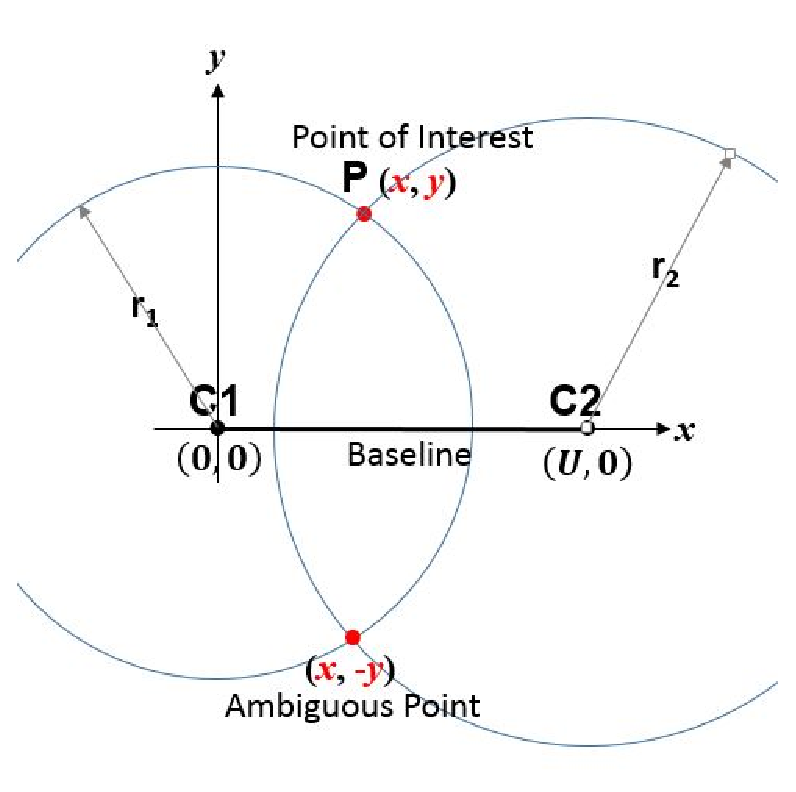
\includegraphics[width=0.5\textwidth]{figures/two_beacon_local}
	\caption{2-D Cartesian true range multilateration (trilateration) scenario}
\end{figure}
Thus, consider the circle centers (or stations) $C1$ and $C2$ in Fig. 1 which have known 
coordinates (e.g., have already been surveyed) and thus whose separation $U$ is known. 
The figure 'page' contains $C1$ and $C2$. If a third 'point of interest' P (e.g., a vehicle or
another point to be surveyed) is at unknown point $(x,y)$  ,then Pythagoras's theorem yields:
\begin{equation}
	\label{equ:ptyhagoras1}
	r_{1}^{2} = x^{2} + y^{2},
\end{equation}
and:
\begin{equation}
	\label{equ:ptyhagoras1}
	r_{2}^{2} = (U-x)^{2} + y^{2},
\end{equation}
therefore robot localisation can be described as a:
\begin{equation}
	\label{equ:two_point_loc}
	\begin{aligned}[t]
		x = \frac{r_{1}^{2}-r_{2}^{2}+U^{2}}{2U},\\
		y = \pm \sqrt{r_{1}^{2}-x^{2}},
	\end{aligned}
\end{equation}
While there are many enhancements, Equation 1 is the most fundamental true range multilateration
relationship.
Aircraft DME/DME navigation and the trilateration method of surveying are examples of
its application. During World War II Oboe and during the Korean War SHORAN used the same 
principle to guide aircraft based on measured ranges to two ground stations.
SHORAN was later used for off-shore oil exploration and for aerial surveying.
The Australian Aerodist aerial survey system utilized 2-D Cartesian true range multilateration.
This 2-D scenario is sufficiently important that the term trilateration is often applied to all
applications involving a known baseline and two range measurements.

The baseline containing the centers of the circles is a line of symmetry.
The correct and ambiguous solutions are perpendicular to and equally distant from
(on opposite sides of) the baseline. Usually, the ambiguous solution is easily identified.
For example, if P is a vehicle, any motion toward or away from the baseline will be opposite 
that of the ambiguous solution; thus, a crude measurement of vehicle heading is sufficient. 
A second example: surveyors are well aware of which side of the baseline that P lies. 
A third example: in applications where P is an aircraft and C1 and C2 are on the ground,
the ambiguous solution is usually below ground.

If needed, the interior angles of triangle C1-C2-P can be found using the trigonometric 
law of cosines. Also, if needed, the coordinates of P can be expressed in a second,
better-known coordinate system—e.g., the Universal Transverse Mercator (UTM) system—provided 
the coordinates of C1 and C2 are known in that second system. Both are often done in surveying
when the trilateration method is employed.
Once the coordinates of P are established, lines C1-P and C2-P can be used as new baselines, and
additional points surveyed.
Thus, large areas or distances can be surveyed based on multiple,
smaller triangles—termed a traverse.

An implied assumption for the above equation to be true is that $r_{1}$ and $r_{2}$ relate to
the same position of P.
When P is a vehicle, then typically $r_{1}$ and $r_{2}$ must be measured within a
synchronization tolerance that depends on the vehicle speed and the allowable vehicle
position error.
Alternatively, vehicle motion between range measurements may be accounted for,
often by dead reckoning.

A trigonometric solution is also possible (side-side-side case). Also, a solution employing 
graphics is possible. A graphical solution is sometimes employed during real-time navigation,
as an overlay on a map. 

%--------------------------------------------------------------------------------------------------
\subsection{Three Cartesian dimensions, three measured slant ranges}
There are multiple algorithms that solve the 3-D Cartesian true range 
multilateration problem directly (i.e., in closed-form) – e.g., Fang.
 Moreover, one can adopt closed-form algorithms developed for pseudo range multilateration.
 Bancroft's algorithm (adapted) employs vectors, which is an advantage in some situations. 
\begin{figure}[htb] 
	\label{fig:three_beacon_local}
	\centering
	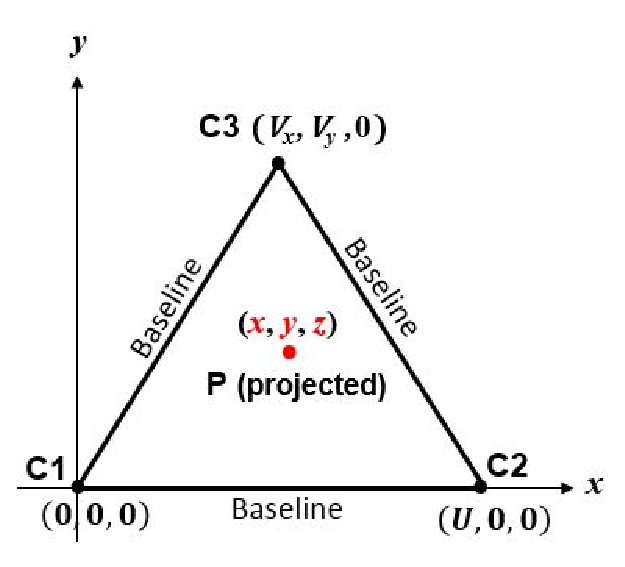
\includegraphics[width=0.5\textwidth]{figures/three_beacon_local}
	\caption{3-D True Range Multilateration Scenario}
\end{figure}
The simplest algorithm corresponds to the sphere centers in Fig. 2. The figure 'page' is the
plane containing C1, C2 and C3. If P is a 'point of interest' (e.g., vehicle) at $(x,y,z)$,
then Pythagoras's theorem yields the slant ranges between P and the sphere centers: 
\begin{equation}
	\label{equ:three_point_pyt}
	\begin{aligned}[t]
		r_{1}^{2}=x^{2}+y^{2}+z^{2},\\
		r_{2}^{2}=(x-U)^{2}+y^{2}+z^{2},\\
		r_{2}^{2}=(x-V_{x})^{2}+(y-V_{y})^{2}+z^{2},\\
	\end{aligned}
\end{equation}
whit assumption that $V^{2} = V_{x}^{2} + V_{y}^{2}$ a following result can be obtained:
\begin{equation}
	\label{equ:three_point_pyt}
	\begin{aligned}[c]
		x = \frac{r_{1}^{2}-r_{2}^{2}+U^{2}}{2U},\\
		y = \frac{r_{1}^{2}-r_{3}^{2}+V^{2}-2V_{x}x}{2v_{y}},\\
		z = \pm \sqrt{r_1{1}^{2}-x^{2}-y^{2}}.
	\end{aligned}
\end{equation}
The plane containing the sphere centers is a plane of symmetry.
The correct and ambiguous solutions are perpendicular to it and equally distant from it, 
on opposite sides.
Many applications of 3-D true range multilateration involve short ranges—e.g.,
precision manufacturing.
Integrating range measurement from three or more radars (e.g., FAA's ERAM) is a 3-D aircraft
surveillance application. 3-D true range multilateration has been used on an experimental 
basis with GPS satellites for aircraft navigation.
The requirement that an aircraft be equipped with an atomic clock precludes its general use.
However, GPS receiver clock aiding is an area of active research, including aiding over 
a network.
Thus, conclusions may change. 3-D true range multilateration was evaluated by the 
International Civil Aviation Organization as an aircraft landing system, but another technique was
found to be more efficient.
Accurately measuring the altitude of aircraft during approach and landing requires many
ground stations along the flight path. 

%--------------------------------------------------------------------------------------------------
\section{Global navigation satellite systems}

%--------------------------------------------------------------------------------------------------
\subsection{Overwiev of GNSS systems}
Satellite navigation systems has become integral part of all applications where mobility plays a
important role (Heinrichs et al., 2005). These functions will be at the heart of the mobile phone
third-generation (3G) networks such as the UMTS. In transportation systems, the presence of
receivers will become as common as seat belts or airbags, with all car manufacturers equipping
their entry-level vehicles with these devices.
As for the past developments, GPS launched a variety of techniques, products and, consequently,
applications and services. The milestone of satellite navigation is the real time positioning and
time synchronization. For that reason the implementation of wide-area augmentation systems
should be highlighted, because they allow a significant improvement of accuracy and integrity
performance. WAAS, EGNOS and MSAS provide over US, Europe, Japan a useful
augmentation to GPS, GLONASS and Galileo services (Mulassano, et al., 2004).
GNSS development has an interesting aspect due to its sensitive nature. Considerable events or
developments are always subject to a couple of differentiators: technological developments and
political decisions.
GPS and Glonass in all stages of improvements are strictly related to those differentiators. The
approval and startup of the European Galileo program is considered by far the most real
innovation. Technological and political decisions in Galileo substantiate that interoperability and
compatibility must be reached in the forthcoming years. Such issues are the true GNSS
improvement for the benefit of institutions and organizations.
GNSS applications in all fields will play a key role, moving its use from the transportation
domain to multimodal use, outdoors and indoors. It is expected that GNSS will increase
significantly the precision in position domain (Lachapelle et al., 2002).
The concept of reference system for navigation is essential since all the applications of GNSS are
related to the coordinate system used. The main application of GNSS is focused on the potential
of to determine the position in the Global reference system any where any time on the Globe in a
simple, fast and cost-effective manner.
The integration between GNSS and other related technologies such as telecommunications
(GSM, GPRS, UMTS), the Geographic Information Systems (GIS) and Inertial Navigation
System (INS), has created numerous applications that needs more time to be discussed in details.
Many research efforts have been exerted in order to find each new applications to promote the
quality of our life using the GNSS benefits (Lohnert et al., 2001; Al-Bayari and Sadoun, 2005).
The GNSS consist of three main satellite technologies: GPS, Glonass and Galileo. Each of them
consists mainly of three segments: 
\begin{enumerate}
	\item space segment,
	\item control segment,
	\item user segment.
\end{enumerate}
These segments are almost similar in the three satellite technologies, which are all together make
up the GNSS. As of today, the complete satellite technology is the GPS technology and most of
the existing worldwide applications related to the GPS technology. The GNSS technology will
become clearer after the operation of Galileo and the reconstruction of Glonass in the next few
years.

%--------------------------------------------------------------------------------------------------
\subsection{GPS components}
The United States Department of Defense (DoD) has developed the Navstar GPS, which is an
all-weather, space based navigation system to meet the needs of the USA military forces and
accurately determine their position, velocity, and time in a common reference system, any where
on or near the Earth on a continuous basis (Wooden, 1985).
GPS has made a considerable impact on almost all positioning, navigation, timing and
monitoring applications. It provides particularly coded satellite signals that can be processed in a
GPS receiver, allowing the receiver to estimate position, velocity and time (Hofmann-Wellenhof
et al., 2001). There are four GPS satellite signals that are used to compute positions in three
dimensions and the time offset in the receiver clock. GPS comprises three main components:
\begin{enumerate}
	\item Space segment: The Space Segment of the system consists of the GPS satellites;
	 see Figure1. These space vehicles (SVs) send radio signals from space as shown in Figure 2.

	\item Control segment: The Control Segment consists of a system of tracking stations located
	around the world. The Master Control facility is located at Schriever Air Force Base
	(formerly Falcon AFB) in the State of Colorado, USA.

	\item User segment: The GPS User Segment consists of the GPS receivers and the user
	community. GPS receivers convert space vehicle (SV) signals into position, velocity, and
	time estimates.
\end{enumerate}

\begin{figure}[htb] 
	\label{fig:gps_constellation}
	\centering
	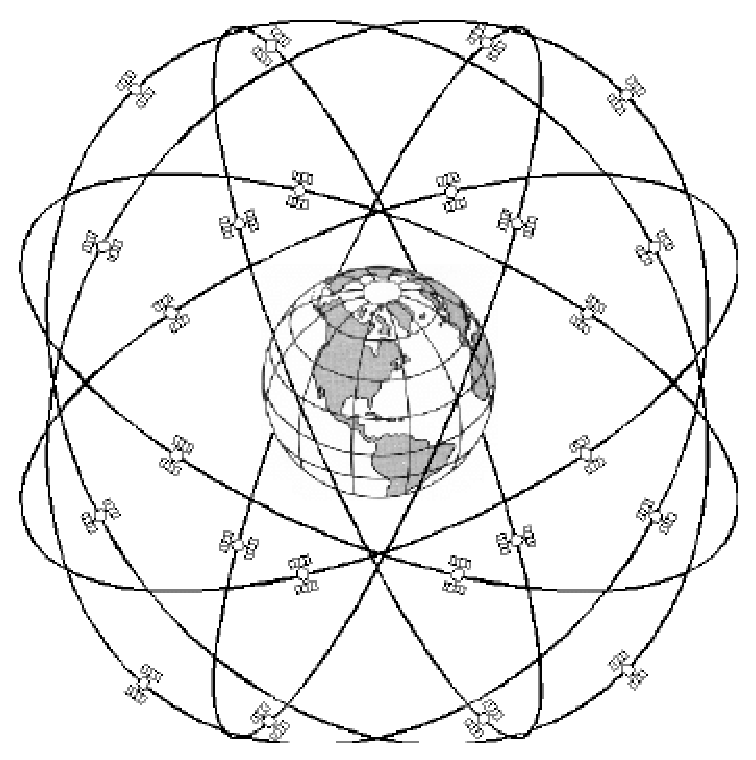
\includegraphics[width=0.5\textwidth]{figures/gps_constellation}
	\caption{GPS Constellation}
\end{figure}

\begin{figure}[htb] 
	\label{fig:gps_signal}
	\centering
	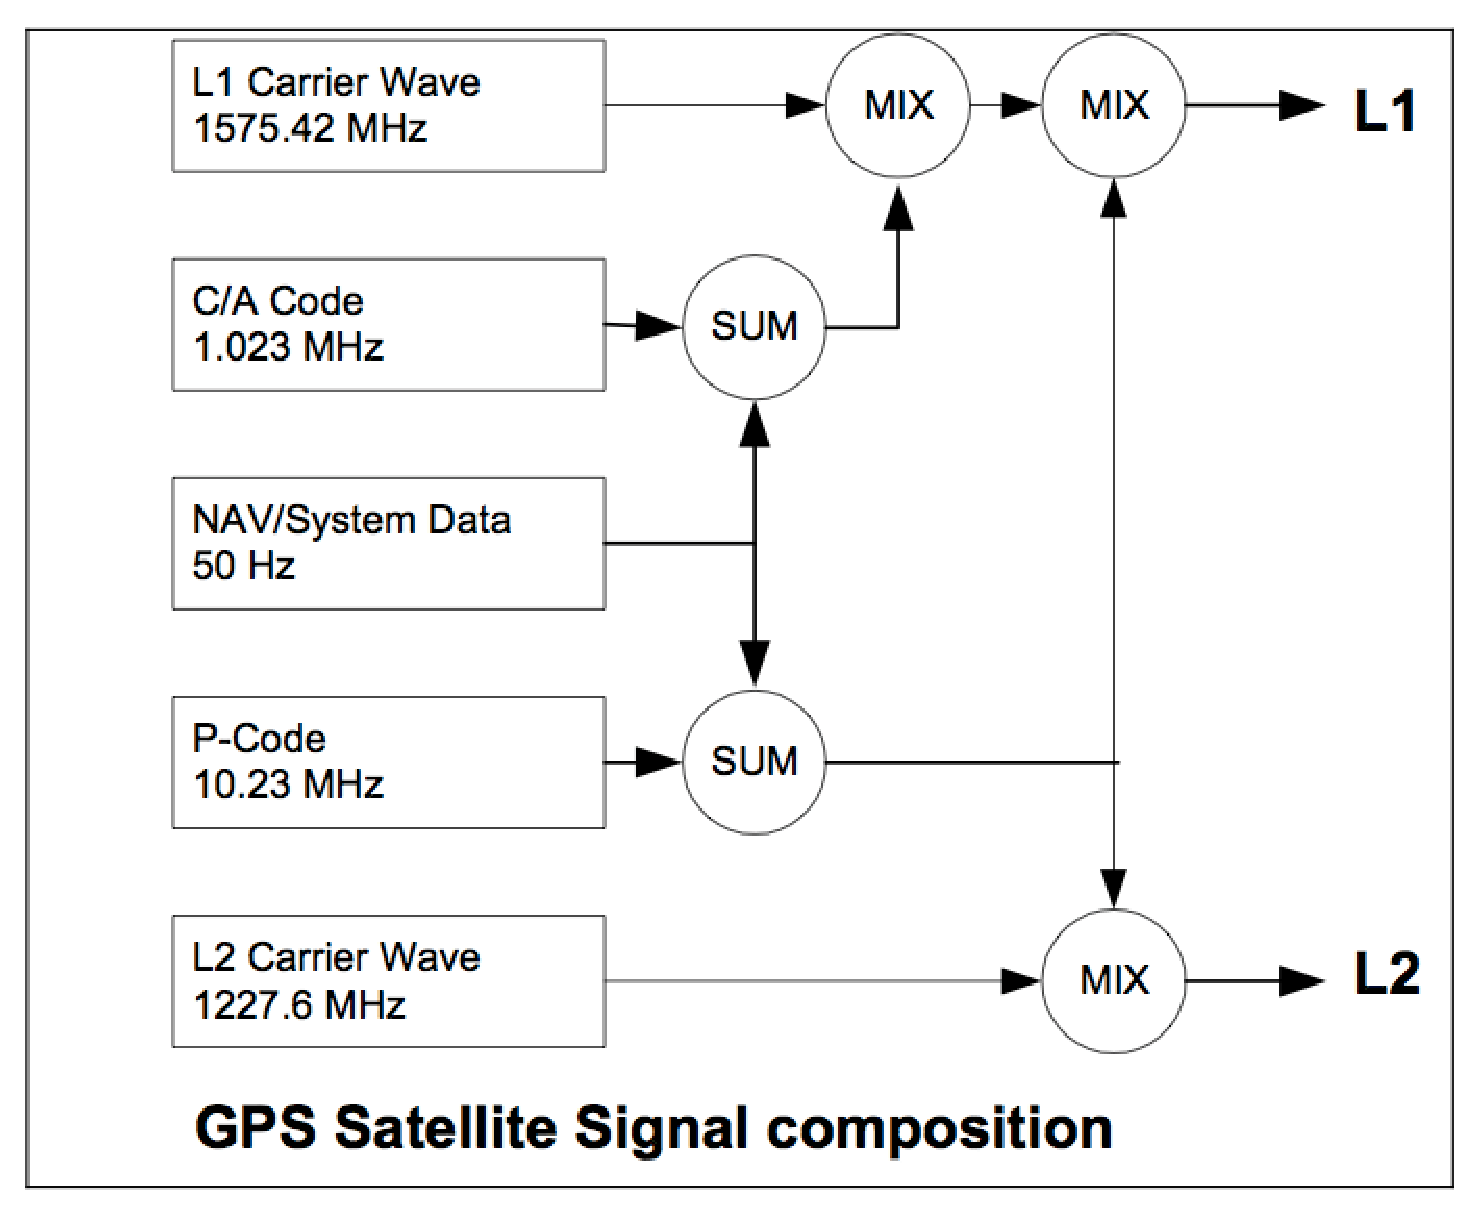
\includegraphics[width=0.8\textwidth]{figures/gps_signal}
	\caption{GPS Satellite Signal}
\end{figure}

The satellites are dispersed in six orbital planes on almost circular orbits with an 
altitude of about 20,200 km above the surface of the Earth, inclined by 55 degree with
respect to the equator and with orbital periods of approximately 11 hours 58 minutes 
(half a sidereal day).
The categories are Block I, Block II, Block IIR (R for replenishment) and Block IIA (A for
advanced) and a further follow-on category Block IIF has also been planned (ICD-GPS, 2003).
Figure 3 shows the main GPS segments.
\begin{figure}[htb] 
	\label{fig:gps_segments}
	\centering
	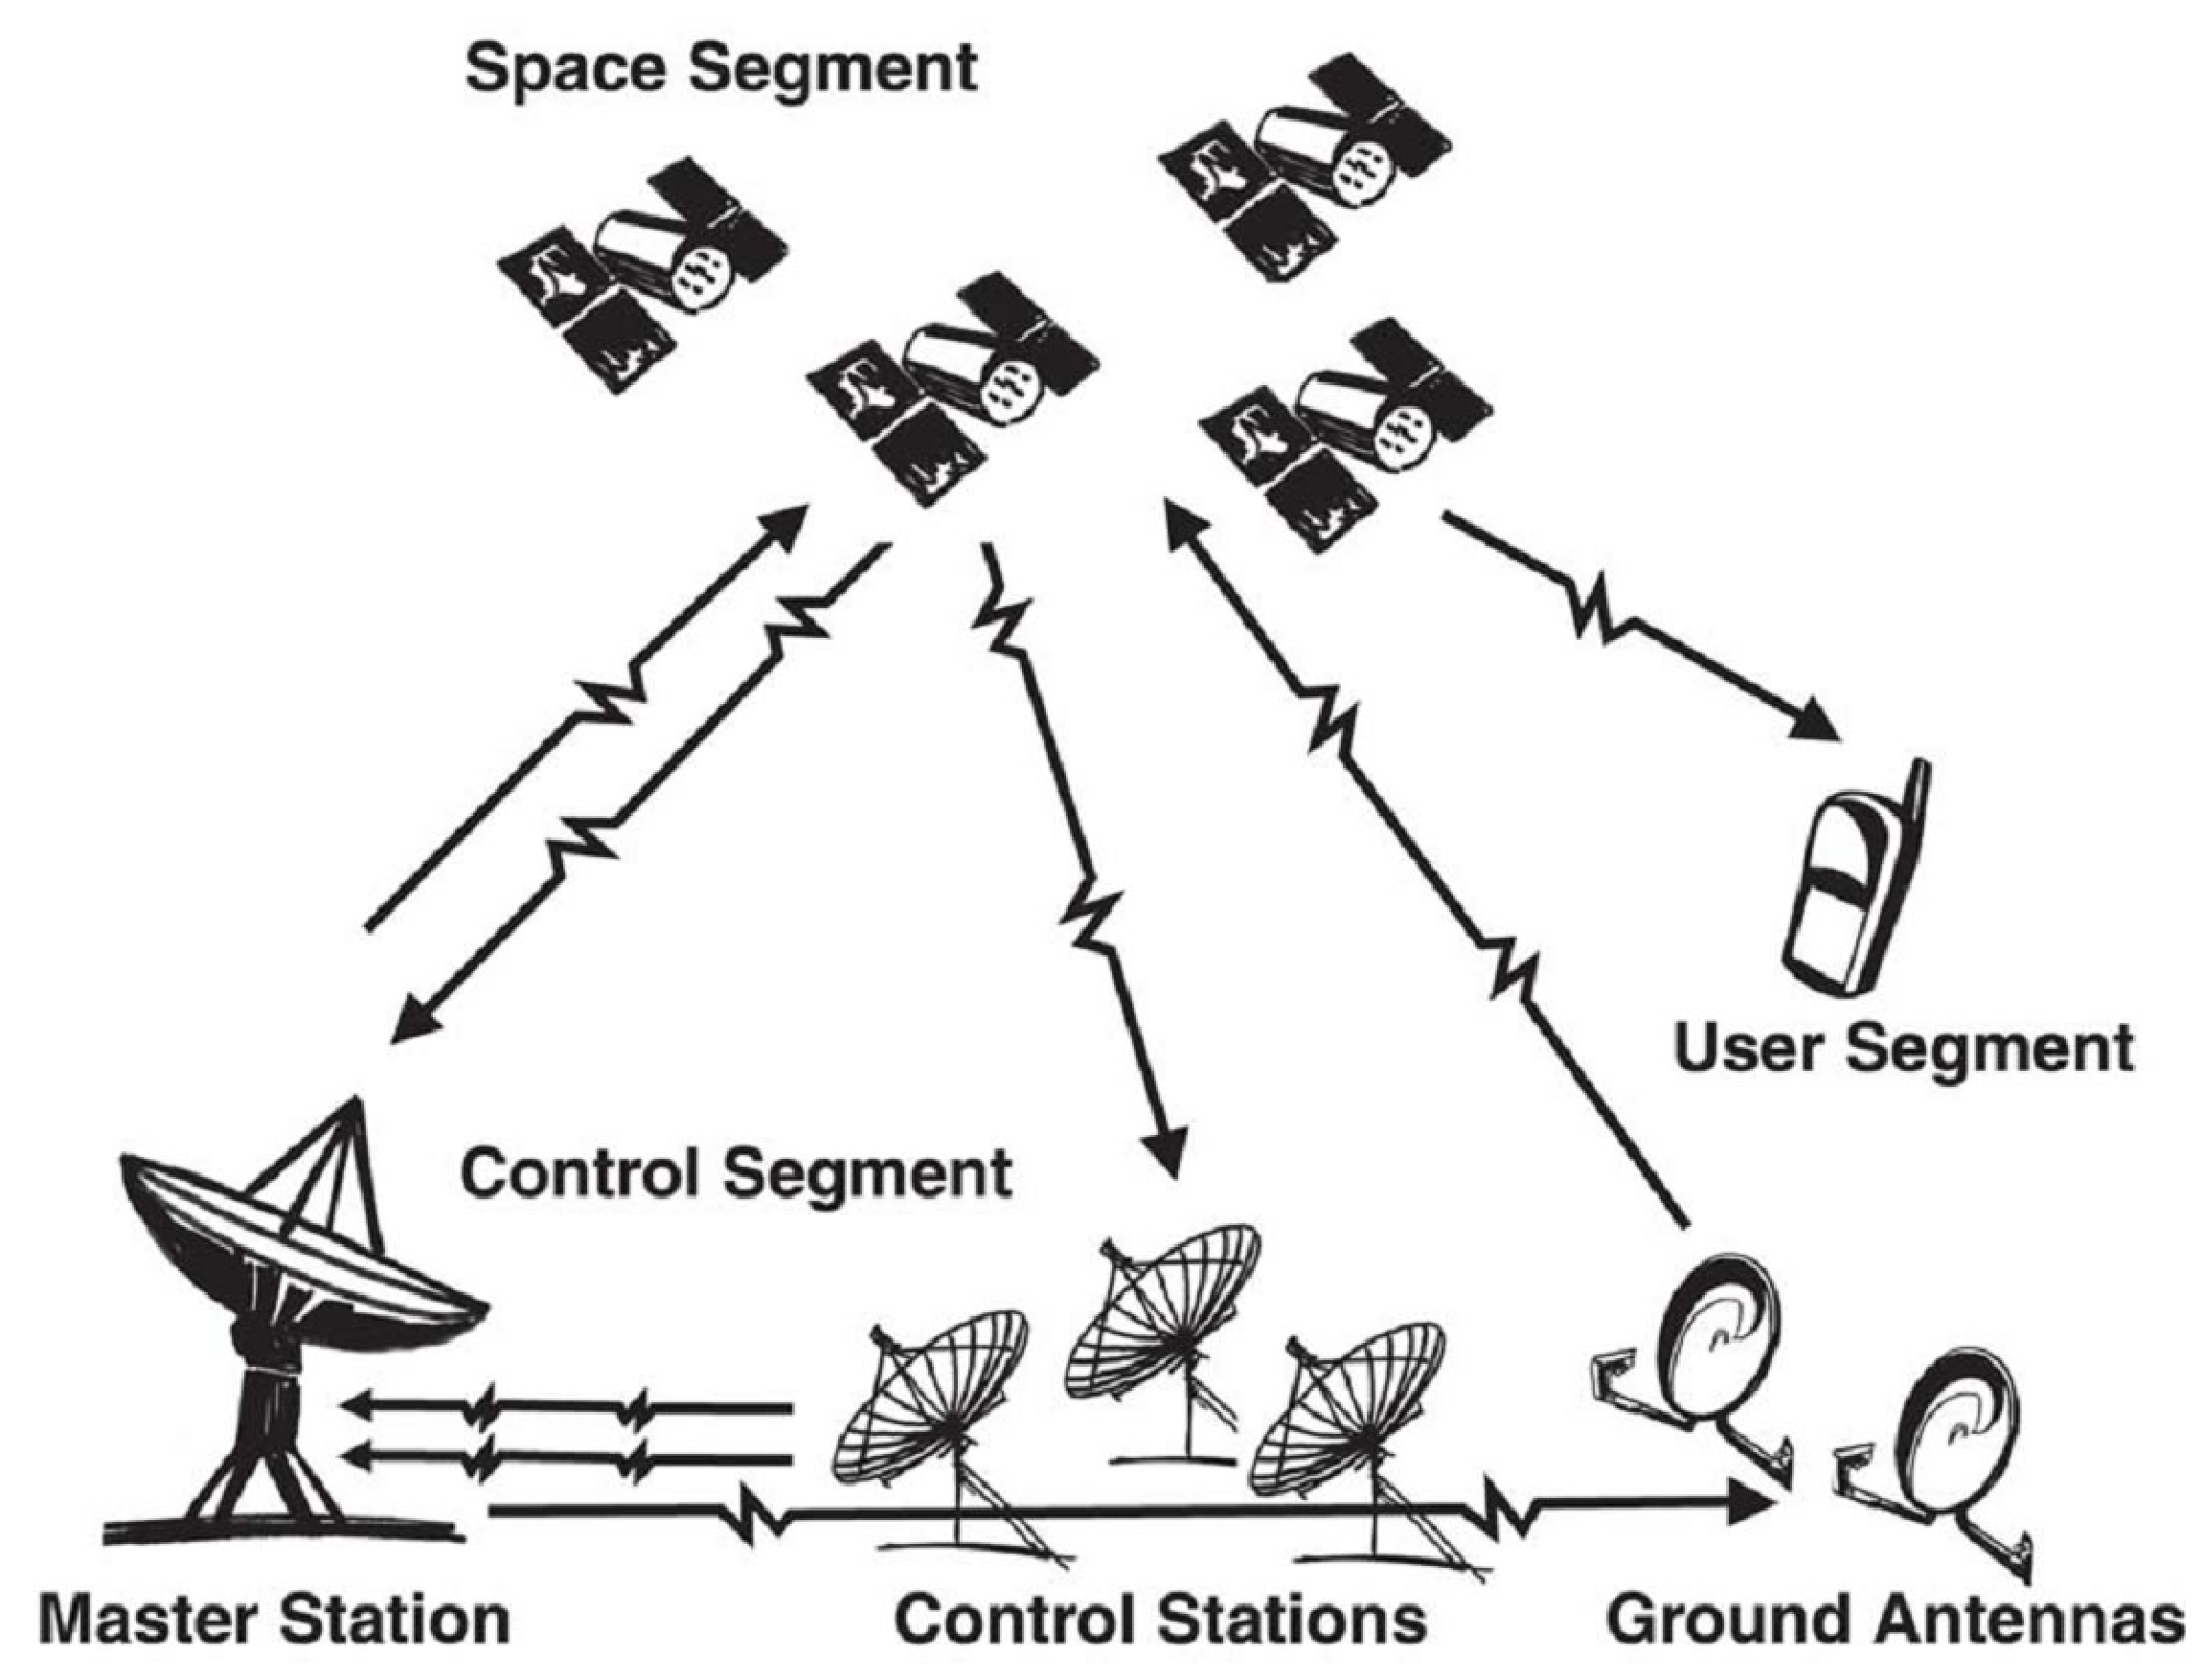
\includegraphics[width=0.8\textwidth]{figures/gps_segments}
	\caption{GPS segments}
\end{figure}


%--------------------------------------------------------------------------------------------------
\subsection{GPS signal}
The generated signals on board the satellites are based or derived from generation of a
fundamental frequency ƒ o =10.23 MHZ (Hofmann-Wellenhof et al., 2001). The signal is
controlled by atomic clock and has stability in the range of 10 - 13 over one day. Two carrier
signals in the L-band, denoted L1 and L2, are generated by integer multiplications of ƒ o . The
carriers L1 and L2 are biphase modulated by codes to provide satellite clock readings to the
receiver and transmit information such as the orbital parameters. The codes consist of a sequence
with the states +1 or -1, corresponding to the binary values 0 or 1. The biphase modulation is
performed by a 180° shift in the carrier phase whenever a change in the code state occurs; see
Figure 4. The clear/access code (C/A-code) and precision code (P-code) are used for the satellite
clock reading, both are characterized by a pseudorandom noise (PRN) sequence. The W-code is
employed to encrypt the P-code to the Y-code when Anti Spoofing (A-S) is applied. The
navigation message is modulated using the two carriers (L1 and L2) at a chipping rate of 50 bps.
\begin{figure}[htb] 
	\label{fig:biphase_modulation}
	\centering
	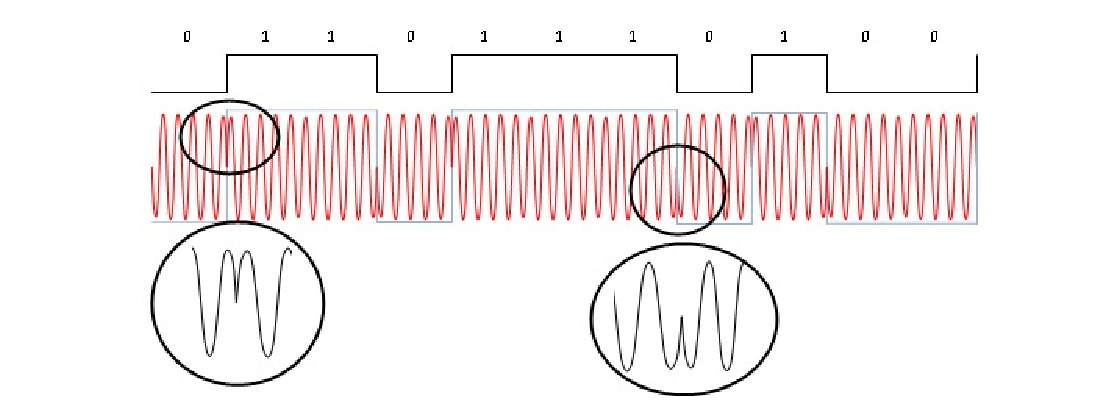
\includegraphics[width=0.8\textwidth]{figures/biphase_modulation}
	\caption{Biphase modulation of carrier}
\end{figure}
It contains information on the satellite orbits, orbit perturbations, GPS time, satellite clock,
ionospheric parameters, and system status messages (Leick, 2003). The modulation of L1 by P-
code, C/A-code and navigation message (D), is done using the quadrature phase shift keying
(QPSK) scheme. The C/A-code is placed on the LI carrier with $90°$ offset from the P-code since
they have the same bit transition epochs. For the L1 and L2 we have:
\begin{equation}
	\label{equ:l1_mod}
	L1(t) = a_{1}P(t)W(t)\cos(2\pi f_{1}t) + a_{1}C/A(t)D(t)\sin(2\pi f_{1}t),
\end{equation}

\begin{equation}
	\label{equ:l1_mod}
	L2(t) = a_{2}P(t)W(t)\cos(2\pi f_{2}t). 
\end{equation}

The signal broadcast by the satellite is a spread spectrum signal, which makes it less prone to
jamming. The basic concept of spread spectrum technique is that the information waveform with
small bandwidth is converted by modulating it with a large-bandwidth waveform (Hofmann-
Wellenhof et al., 2001).
The generation of pseudo random sequence (PRN) in the code is based on the use of an
electronic hardware device called tapped feed back shift register (FBSR). This device can
generate a large variety of pseudo random codes, but in this way the generated code repeat it self
after some very long time. The receiver could distinguish the signals coming from different
satellites because the receiving C/A code (the Gold code), has low cross-correlation and is
unique for each satellite (Leick, 2003).
The navigation message consists of 25 frames with each frame containing 1500 bit and each
frame is subdivided into 5 sub-frames with 300 bit. The information transmitted by the
navigation message is periodically updated by the control segment.

%--------------------------------------------------------------------------------------------------
\subsection{Modernized GPS}
Due to the vast civil applications of GPS technology during the past decade or so and due to the
new technologies used in the satellite and receivers, the U.S government has decided to extend
the capabilities of GPS to give more benefits to the civil community. In addition to the existing
GPS signals, new signals will be transmitted by GPS satellite; see Figure 5. Moreover, this will
increase the robustness in the signals and improve the resistance to signal interference. This
definitely will lead to a better quality of service (QoS). The new signals added to the GPS
(Fontana et al., 2001), are: (i) a new L5 frequency in an aeronautical radio navigation service
(ARNS) band with a signal structure designed to improve aviation applications, (ii) C/A code to
L2C carrier (L2 civil signal ), and (iii) a new military (M) code on L1 and L2 frequency for the
DoD has been added. It has the potential to track signal even in poor conditions where the C/A
code tracking on L1 would not be possible. The new military code will be transmitted from the
Block IIR-M and IIF satellites (Betz, 2002).

It is well known that the presence of dual frequency measurements (L1 and L2) has good
advantages to eliminate the effect of the ionosphere and enhance the ambiguity resolution
especially for the high precision measurements (Liu and Lachapelle, 2002). High-end civil dual
frequency systems will be based on L1 CA-code and the newly designed L2 C-code. In the
coming few years the receivers will become more complex in order to allow tracking the new
civil code on L2 and tracking the encrypted P on L2 (A-S).
The frequency of L5 is 1176.45MHz, with chipping rate of 10.23 MHz similar to P- code. The
high chipping rate of L5 code will provide high performance ranging capabilities and better code
measurement than L1 C/A code measurements (Dierendonck and Hegarty, 2000).
L2 has a better correlation protection with respect to L1 since it has a long code. This will be
useful in severe conditions where the GPS signals are weak such as navigation in urban, indoor,
and forested areas.
The old codes and the new codes (Millitary and civil), on the L1, L2 and L5 need more
advanced modulation that better share existing frequency allocations with all signals by
increasing spectral separation, and hence conserve the spectrum. Consequently, binary offset
carrier (BOC) is used for the Military code modulations (Betz, 2002).

\begin{figure}[htb] 
	\label{fig:modernized_gps_signal}
	\centering
	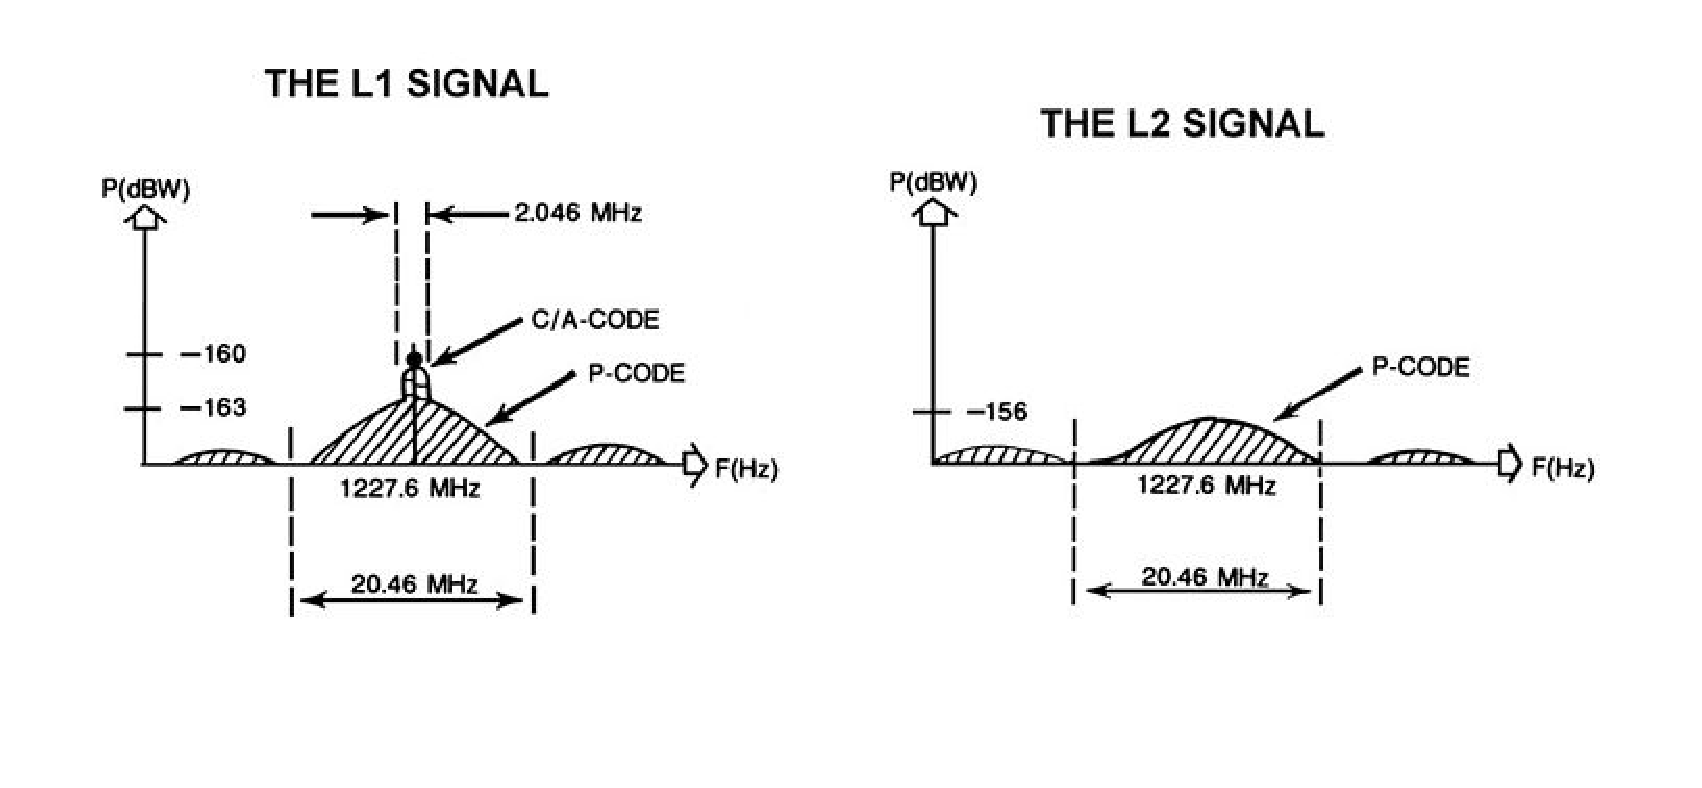
\includegraphics[width=0.8\textwidth]{figures/modernized_gps_signal}
	\caption{Modernized GPS signals}
\end{figure}

%--------------------------------------------------------------------------------------------------
\subsection{Alternatives to GPS}
The GLONASS (GLObal NAvigation Satellite System or “GLObalnaya NAvigatsionnaya
Sputnikovaya Sistema”) is nearly identical to GPS. Glonass satellite-based radio-navigation
system provides the positioning and timing information to users. It is operated by the Ministry of
Defense of the Russian Federation (GLONASS-ICD, 2002).
Glonass space segment is consist of 24 satellites, equally distributed in 3 orbit separated by 120 o
in the equatorial plane. Satellite orbital altitude is about 19,130 km above the ground surface.
This results in an orbital period of 11:15:44 corresponding to 8/17 of a sidereal day.
The future of GLONASS seems uncertain due to economic problems facing the Russian
Federation. The number of operational satellites was steadily decreasing over the past few years.
The launch of three new GLONASS satellites in December 1998 was the first launch after a
lapse of 3 years.
As of January 2006, a total of 10 GLONASS satellites are operational. The oldest of the still
active satellites was launched in October, 2000. According to Russian officials the GLONASS
system shall again be restored by 2008.

GALILEO is Europe’s initiative for a state-of-the-art global navigation satellite system,
providing a highly accurate, guaranteed global positioning service under civilian control. Galileo
will be not too different from the other GNSS parts (modernized GPs and Glonass (Salgado et
al., 2001). It will provide autonomous navigation and positioning services, but at the same time
will be interoperable with the two other global satellite navigation systems; the GPS and
GLONASS. A user will be able to take a position with the same receiver from any of the
satellites in any combination. By providing dual frequencies as standard, however, GALILEO
will deliver real-time positioning accuracy down to the meter range. It will guarantee availability
of the service under all, but the most extreme circumstances and will inform users within seconds
of a failure of any satellite. This will make it appropriate for applications where safety is vital,
such as running trains, guiding cars and landing aircraft. The combined use of GALILEO and
other GNSS systems can offer much improved performance for all kinds of users worldwide.
GALILEO is expected to be in operation by the year 2008. The first satellite of Galileo system
(GIOVE A) has already been lunched in 27 th December 2005.

%--------------------------------------------------------------------------------------------------
\subsection{Coordinate system}
The definition of reference coordinate system is crucial for the description of satellite motion,
the modeling of observable and the interpretation of results.
Reference coordinate system in satellite geodesy is global and geocentric by nature since 
satellite motion refers to the center of mass of the earth 
(Seeber, 2003; Hofmann-Wellenhof et al., 2001).
In satellite geodesy, two reference systems are required:
\begin{enumerate}
	\item space-fixed, inertial reference system for the description of satellite motion,
	\item earth-fixed, terrestrial reference system for the positions of the observation stations
		and for the description of results from satellite geodesy.
\end{enumerate}
The positioning with using GNSS depends mainly on knowing the satellite coordinates. 
The position of the receiver is calculated with respect to the instant position of the satellite. 
By considering the range vector relation between satellite and receiver, 
the coordinate of the satellite and receiver should be expressed in the same coordinate system.
In satellite geodesy, the two systems are used and the transformation parameters between the
space fixed and earth fixed are well known and used directly in the GNSS receiver and post
processing software to compute the position of the receivers in the earth fixed system.
Terrestrial reference system is defined by convention with three axes, where Z-axis coincides
with the earth rotation axis as defined by the Conventional International Origin (CIO). The X-
axis is associated with the mean Greenwich meridian, and the Y-axis is orthogonal to both Z and
X axes and it completes the right-handed coordinate system, Fig. 9. One example of the
terrestrial reference system is the WGS84. GPS has used the WGS84 as a reference system
(Leick, 2003), and with WGS84 associated a geocentric equipotential ellipsoid of revolution.
16The basic idea, in geodesy, behind using the reference ellipsoids is that they fit the real
shape of the earth.
Another example of terrestrial reference frame is the International Terrestrial Reference Frame
(ITRF), which is established by Central Bureau of the International Earth Rotation Service
(IERS). The ITRF is regularly updated and is more accurate than WGS84, but the difference
between WGS84 and ITRF is now in the order of a few centimeters. This difference is mainly
due to the difference between the reference stations used by each system when it is realized.
Both systems are geocentric and the transformation parameters between them are regularly
published by IERS.
The representation of position in geocentric Cartesian coordinates (X, Y and Z) has less
significance in navigation. Hence, the ellipsoidal representation (longitude, latitude and height
above the ellipsoid) are more commonly use for coordinate representation.
\begin{figure}[htb] 
	\label{fig:ecef_coordinate}
	\centering
	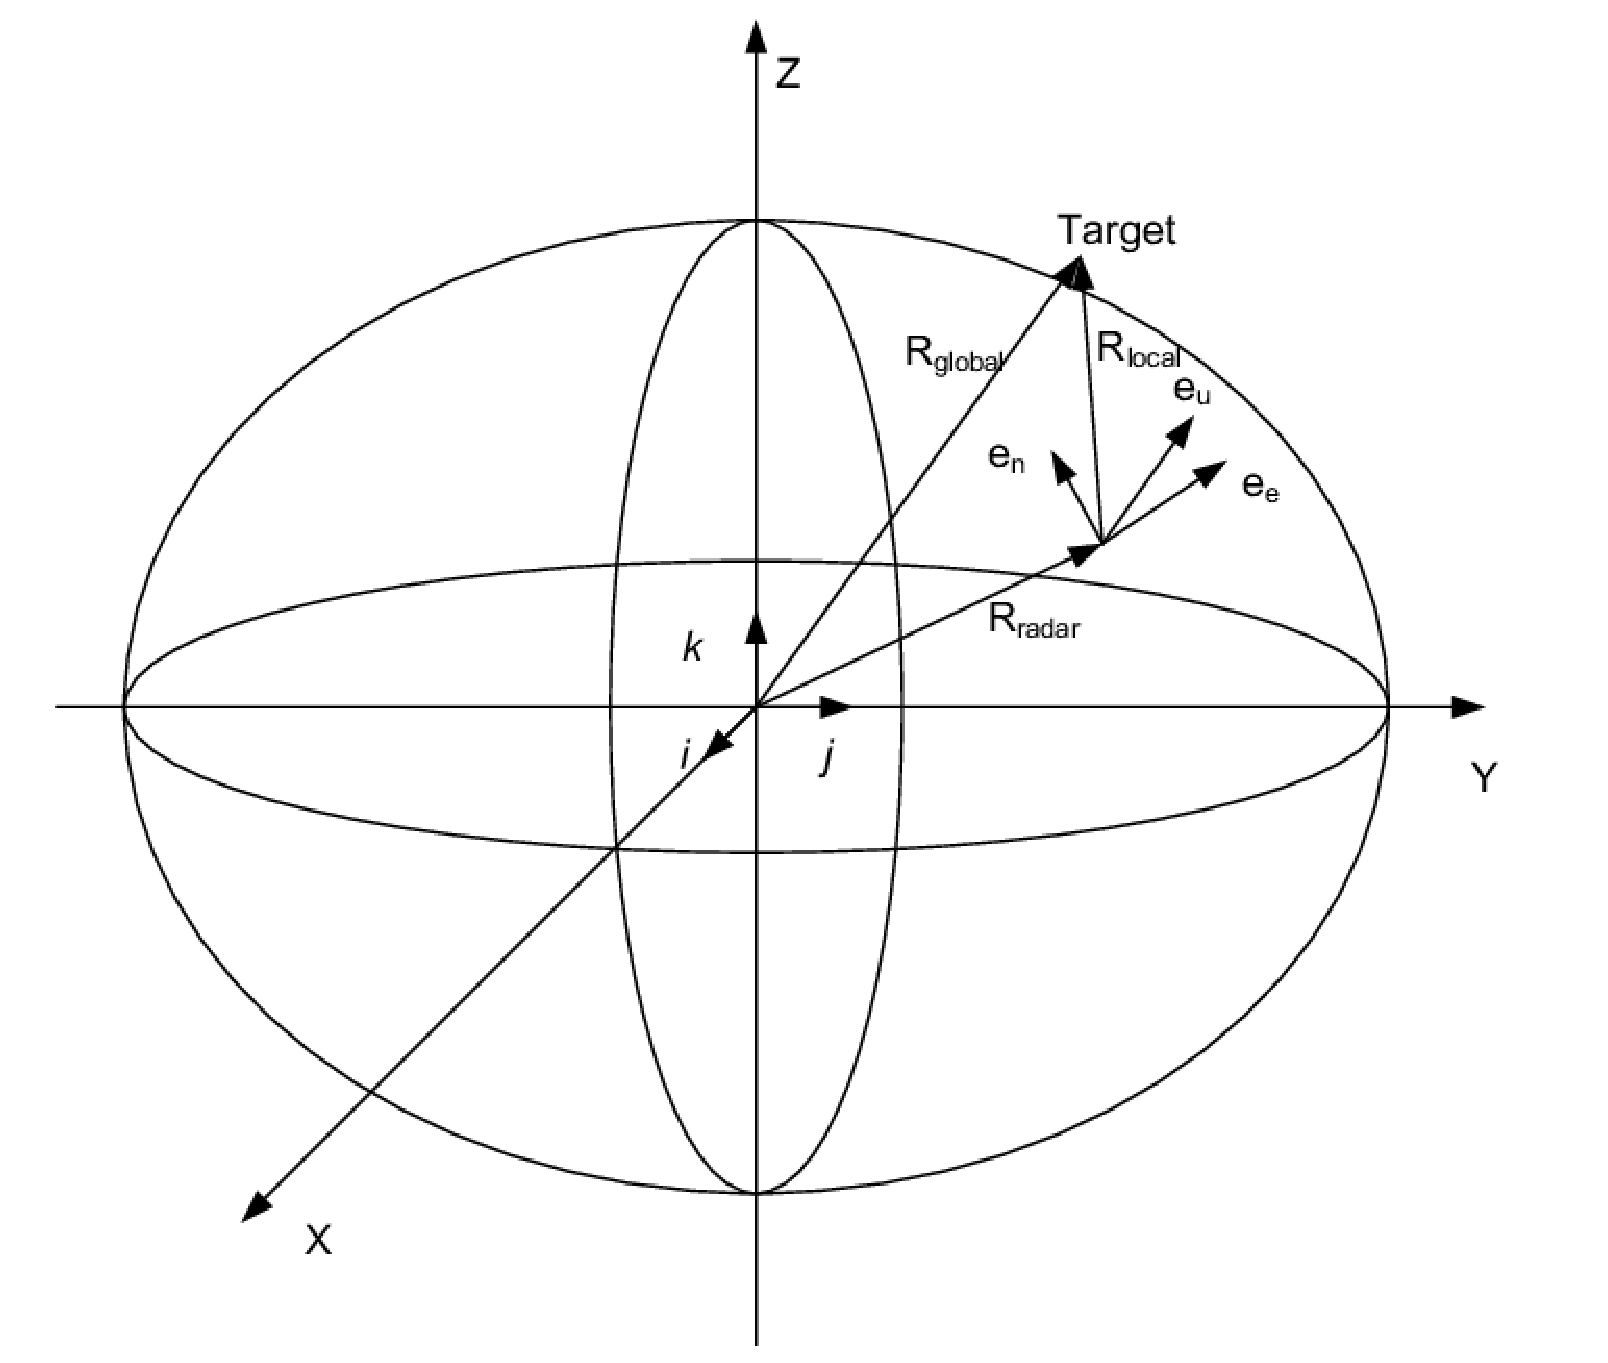
\includegraphics[width=0.8\textwidth]{figures/ecef_coordinate}
	\caption{ECEF coordinate system and ellipsoidal coordinates}
\end{figure}
The relation between Cartesian coordinate $(X,Y,Z)$ and ellipsoidal coordinates 
$( \phi , \lambda , h )$ are described by the following formulas:
\begin{equation}
	\label{equ:ecef}
	\begin{aligned}[c]
		X = (N+h)\cos(\phi)\cos(\lambda),\\
		Y = (N+h)\cos(\phi)\sin(\lambda),\\
		Z = (\frac{b^{2}}{a^{2}}N+h)\sin(\phi),
	\end{aligned}
\end{equation}
where $a$ and $b$ are the semi axes of the ellipsoid and $N$ is the radius of curvature in 
prime vertical and is obtained by the following expression:
\begin{equation}
	\label{equ:curvature}
	N = \frac{a^{2}}{\sqrt{a^{2}cos^{2}(\phi)+b^{2}sin^{2}(\phi)}}.
\end{equation}
The Cartesian coordinate of WGS84 is called also
ECEF (Earth Centered Earth-Fixed) coordinate system.
As mentioned above, the realization of the reference frame depends on the coordinates of ground
reference stations. The Galileo Terrestrial Reference Frame (GTRF) is expected to be similar to
ITRF, but will be based on the coordinates of the Galileo ground stations. The differences
between WGS84, ITRF and the GTRF are expected to be in the order of a few centimeters. The
two coordinate systems are compatible, and the accuracy obtained is good enough for most of the
applications including navigation. For high precise measurements and for centmetric accuracy
between the various systems, the transformation parameters are expected to be published by the
geodetic service providers such as IERS. Glonass uses the PZ90 as a reference coordinate system
which is basically a ECEF system. The transformation parameters between PZ90 and WGS84 is
published by IERS (Leick, 2003).


%--------------------------------------------------------------------------------------------------
\subsection{Code and phase pseudorange measurements}
Code correlation technique is used to measure the time difference between the received and
generated replica code. The range could be formulated as follows:
\begin{equation}
	\label{equ:range}
	R_{R}^{S} = c [(t_{R(GNSS)}-\delta_{R})-( t_{S(GNSS)}-\delta_{S})],
\end{equation}
where $\delta_{S}$ is the satellite clock offset  and $\delta_{R}$ is the receiver clock offset.
A high stability atomic clock is generally used on board of the satellite, so $\delta_{S}$ is 
small and could be modeled by a polynomial with the coefficients being transmitted in the 
navigation message. However, the receiver clock offset $\delta_{R}$ is large and is treated as
 unknown to be estimated in the function:
\begin{equation}
	\label{equ:reciever_error}
	R_{R}^{S} = c \Delta t_{GNSS} + c( \delta_{S} - \delta_{R}) = \rho + c  \Delta \delta,
\end{equation}
where $\rho$ is the true distance between satellite and receiver and its expressed by the vector in
reference geocentric coordinate system as:
\begin{equation}
	\label{equ:distance_geocentric}
	\rho = \sqrt{(X_{S}-X_{R})^{2}+(Y_{S}-Y_{R})^{2}+(Z_{S}-Z_{R})^{2}}.
\end{equation}
Phase pseudo range is based on the measurements of phase difference between the received and
generated signal $\varphi \theta_{R}^{S}$ at the receiver. The received carrier is
Doppler shifted due to the motion of satellite (Hofmann-Wellenhof et al., 2001).
In order to calculate the range using phase measurement, we have to add to $\varphi \theta_{R}^{S}$ 
the number of cycles between the satellite and the receiver, which is an ambiguous value and is
often called ambiguity (N). By considering the initial phase errors of the satellite and receiver
due to their clocks, the mathematical model of phase pseudo range can be expressed by:
\begin{equation}
	\label{equ:phase_pseudorange}
\delta \varphi_{R}^{S}+N = -\frac{f}{c}\rho = f\delta_{S} + f\delta{R}.
\end{equation}
If we rearrange the above equation and use $\Phi = -\delta \phi_{R}^{s}$ and 
$\Delta \delta = \delta_{S} - \delta_{R}$ , the it becomes similar to the code pseudo range
equation, but with the additional the ambiguity value $(N)$:
\begin{equation}
	\label{equ:phase_pseudorange2}
	\lambda \Phi = \rho + c \Delta \delta + \lambda  N,
\end{equation}
where $\lambda$ is the wave length.

%--------------------------------------------------------------------------------------------------
\subsection{GNSS observable errors}
The code and phase measurements are affected by noise and errors due to the propagation of
signals through atmospheric layers and due to the noise measurements. These errors can
described briefly as below:

Satellite clock error: This can be modeled by the polynomial coefficients transmitted in the
navigation message with respect to a reference time (e.g. GPS).
\begin{equation}
	\label{equ:sat_clock_error}
	\delta S = a_{0} + a_{1}(t-t_{0}) + a_{2}(t- t_{0} )^{2}.
\end{equation}

Orbital error: This can be eliminated by differential positioning. Precise orbits could be
obtained in near real time via Internet from the services centers such as International GNSS
Service (IGS).

Ionospheric error: This error is modeled or eliminated by using the linear combination of two
or multiple frequencies (Julien et al., 2004b). The relation between the ionospheric effect on the
future GNSS (L5, L2 and L1 for GPS; E5a, E5b and E1 for GALILEO) using the triple
frequency could be written as follows:
\begin{equation}
	\label{equ:ionospheric_error}
	\begin{aligned}[c]
		\lambda_{1} \Phi_{1} = \rho + c \Delta \delta + \lambda_{1} N - I_{L1},\\
		\lambda_{2}\Phi_{2} = \rho + c \Delta \delta + \lambda_{2} N - 
		\frac{f_{1}^{2}}{f_{2}^{2}}I_{L1},\\
		\lambda_{3}\Phi_{3} = \rho + c \Delta \delta + \lambda_{3} N - 
		\frac{f_{1}^{2}}{f_{3}^{2}}I_{L1},
	\end{aligned}
\end{equation}
where $Ionosphere = I_{L1}$.
The effect of ionosphere on GNSS measurement is of special interest in solving the ambiguity
number N (Liu and Lachapelle, 2002). Having multiple frequency can give more advantages for
ionosphere models to estimate the first and second order effect of the ionosphere. Moreover, it
allows more possibilities in ambiguity resolution process (Zhang, et al., 2003). Ionosphere could
also be modeled using the ionospheric coefficient transmitted by the navigation message.

The troposphere: This consists of two layers: Wet layer (up to 10 km above the surface of
ground), and dry layer from 10 to 40 km above the ground. Troposphere causes a delay in both
the code and carrier observations. Since it is not frequency dependent, it cannot be canceled out
by using dual frequency measurements but it can, however, be successfully modeled.
Tropospheric models depend on empirical models by considering all values of temperature,
pressure, relative humidity and mapping function. Examples of such models are the Hopfield,
and Saastamoninen models.

Receiver clock error: This is due to using non-precise clock in the receiver (e.g. quartz clock),
which causes offset and drift in the receiver clock and GNSS reference time. This error is treated
as unknown in the pseudo range computations. The clock receiver error could be eliminated in
double difference equation as shown in the follow section.

Multipath: This is caused by multiple reflections of the signals at the receiver or at the satellite
due to multiple paths taken by the signal to arrive to the destination. The best way to reduce
multipath phenomenon is to choose the site away from reflection surface (such as buildings, cars,
trees, etc), and by appropriate antenna design. Carrier phase are less affected by multipath
propagation than code ranges, because multipath is frequency dependent. The multipath error
could reach to a one meter level. The elimination of multipath is possible by selecting an antenna
that takes advantages of the signal polarization.

%--------------------------------------------------------------------------------------------------
\subsection{Single Point Positioning}
The basic concept of point position depends on the trilatration between the receiver and satellite.
Range measurements from 4 satellites is needed to determine the four unknown $X, Y, Z$ and
receiver clock offset $\Delta \delta$. The analytical solution for receiver A and 4 
satellites could be written as below :
\begin{equation}
	\label{equ:single_point}
	R_{A}^{1} = \sqrt{(X^{1}(t)-X_{A})^{2}+(Y^{1}(t)-Y_{A})^{2}+(Z^{1}(t)-Z_{A})^{2}}.
\end{equation}
Generally, linearization respect to approximate position of the receiver is needed to resolve such
model, where the range R is measured by the receiver and the coordinate of satellite is extracted
from the navigation message. The unknowns in the above equation are $X, Y, Z$ and the clock
error $\Delta \delta$ . In case of observing more than 4 satellites, the least square adjustment
is performed  to estimate the unknowns.
Hence, coordinates of the receiver and time offset could be obtained directly in real time with
one epoch measurement. Geometric information could be obtained from equation model as
PDOP which indicates the quality of the solution with respect to satellite geometry. Bad satellite
distribution give large PDOP. Due to un-modeled errors in pseudo range such as ionosphere,
troposphere, and orbital errors, the accuracy level of absolute positioning is within 10 meter.

%--------------------------------------------------------------------------------------------------
\subsection{Observable difference}
By considering all the systematic and random errors on the observation, we can write the math
model for observable difference for code and phase measurements, respectively, as below:
\begin{equation}
	\label{equ:diff_r}
	R^{1}_{A}(t_{0}) = \rho^{1}_{A}(t_{0})+\Delta \rho^{1}_{A}(t_{0}) + c \delta^{1}(t_{0})-
	c\delta_{A}(t_{0}) + I_{A} + T_{A} + \varepsilon,
\end{equation}

\begin{equation}
	\label{equ:diff_lambda}
	\lambda \phi^{1}_{A}(t_{0}) = \rho^{1}_{A}(t_{0}) + \Delta \rho^{1}_{A}(t_{0}) 
	+ \lambda N^{1}_{A} + c \delta^{1}(t_{0}) - c \delta_{A}(t_0) - I_{A} + T_{A} + \varepsilon,
\end{equation}
where $\Delta \rho_{R}^{S}$ is the orbital error, $I$ is the ionosphere error, $T$ is the
troposphere error and $\varepsilon$ represents other types of noise and errors such as the
ones due to multipath.

Using two receivers A and B and satellite (1), we can perform Single Differences (SD). In SD
the orbital error and satellite clock error are cancelled.
By using two receivers and two satellites (1, 2), we can perform Double Differences (DD).
In DD the clock receiver error is cancelled. By using two receivers, two satellites and two 
consequent epochs, we can perform Triple Differences (TD). In TD the ambiguity is cancelled.
\begin{equation}
	\label{equ:cancellation}
	\begin{aligned}[c]
		SD = \lambda \phi_{AB}^{1}(t) = \lambda \phi_{B}^{1}(t)-\lambda \phi_{A}^{1}(t) =
		\rho^{1}_{AB}(t) + \lambda N^{1}_{AB}- c\delta_{AB}(t_{0}),\\
		DD = \phi_{AB}^{12}(t) = \frac{1}{\lambda}\rho^{12}_{AB}(t) + N^{12}_{AB},\\
		TD = \phi_{AB}^{12}(t_{12}) = \frac{1}{\lambda}\rho^{12}_{AB}(t_{12}
	\end{aligned}
\end{equation}
As we see, most of systematic errors are cancelled or reduced with using the observable
differences. Consequently, the accuracy of position computation will be improved after
eliminating or reducing of these biases. Solution obtained in DD with ambiguity can provide a
precision to the centimeteric level.

%--------------------------------------------------------------------------------------------------
\subsection{Differential position}
There is an increase interest in differential positioning due to the numerous advantages of
wireless communications and networks. Most of errors that affect GNSS are common between
the receivers, which observe the same set of satellites (Leick, 2003; Hofmann-Wellenhof et al.,
2001). Thus, by making differential measurement between two or more receivers, most of these
errors could be cancelled.
The basic concept of differential position is the calculation of position correction or range
correction at the reference receiver and then sending this correction to the other receiver via
radio link. This way most of errors are cancelled; see Fig.11. The transmitted correction could be
of several types: the position or pseudo range correction, the carrier smoothed pseudo range
correction, and the carrier phase correction. The mathematical model of DGNSS could be written
as shown below. Two receivers are used, where receiver A is installed at known reference station
and B is rover/moving receiver. Pseudo range at A is given by:
\begin{equation}
	\label{equ:diferential_pos1}
	R^{1}_{A}(t_{0}) = \rho^{1}_{A}(t_{0}) + \Delta \rho^{1}_{A}(t_{0}) + c \delta^{1}(t_{0})
	- c \delta_{A}(t_{0}),
\end{equation}

\begin{equation}
	\label{equ:diferential_pos2}
	PRC^{1}(t_{0}) = -R^{1}_{A}(t_{0}) + \rho^{1}_{A}(t_{0}) = -\Delta \rho^{1}_{A}(t_{0}
	- c \delta^{1}(t_{0}) + c \delta_{A}(t_{0}).
\end{equation}

\begin{figure}[htb] 
	\label{fig:gps_correction}
	\centering
	
\includegraphics[width=0.8\textwidth]{figures/gps_correction}
	\caption{Modernized GPS signals}
\end{figure}
We have to add the range rate correction for an arbitrary epoch (t).
\begin{equation}
	\label{equ:range_rate_correction}
	PRC^{1}(t) = PRC^{1}(t_{0}) + RRC^{1}(t_{0})(t-t_{0}),
\end{equation}
where $(t-t_{0})$, is called the latency due to transmission time between  the reference and 
the rover receiver.
The pseudo range at receiver B could be written as:
\begin{equation}
	\label{equ:reciever_pseudorange}
	R_{B}^{1}(t) = \rho^{1}_{B}(t) + \Delta \rho^{1}_{B}(t) + c \delta^{1}(t)- c \delta_{B}(t),
\end{equation}
By adding the pseudo range from reference station, we obtain:
\begin{equation}
	\label{equ:pseudorange_with_ref1}
	R_{B}^{1}(t)_{corr} = R_{B}^{1}(t) + PRC^{1}(t) = \rho B^{1}(t)+(\Delta \rho B^{1}(t)-
	\Delta \rho^{1}_{A}(t)) - ( c \delta_{B}(t) - c \delta_{A}(t)),
\end{equation}
\begin{equation}
	\label{equ:pseudorange_with_ref2}
	R_{B}^{1}(t)_{corr} = \rho^{1}_{B}(t) - c \Delta \delta_{AB}(t).
\end{equation}
As we see the orbital error is cancelled and the satellite clock error is eliminated. We can also
transmit the phase correction to the rover receiver. In this case we have to add another unknown;
the ambiguity N, to the equations. The phase range correction between the reference and the
rover receiver when applying the same above procedure will be given by:
\begin{equation}
	\label{equ:phase_label_corr}
	\lambda \phi B^{1}(t)_{corr} = \rho B^{1}(t)+\lambda \Delta N^{1}_{AB}-c\Delta \delta_{AB}(t),
\end{equation}
DGNSS with phase range correction is used for most precision Real-Time Kinematics (RTK).
But the ambiguity should be resolved or fixed by using the On The Fly (OTF) techniques. In
phase measurement technique the precision obtained will be at the centimeter level. Modeling
the ionosphere and troposphere will eliminate or reduce the errors in DGNSS. This method gives
more possibilities to obtain high accuracy in point positioning using one receiver.
